\documentclass[border=10pt]{standalone}
\usepackage{tikz}
\usetikzlibrary{shapes.geometric, arrows.meta, positioning, calc}
\usepackage[ruled,vlined,linesnumbered]{algorithm2e}

\begin{document}

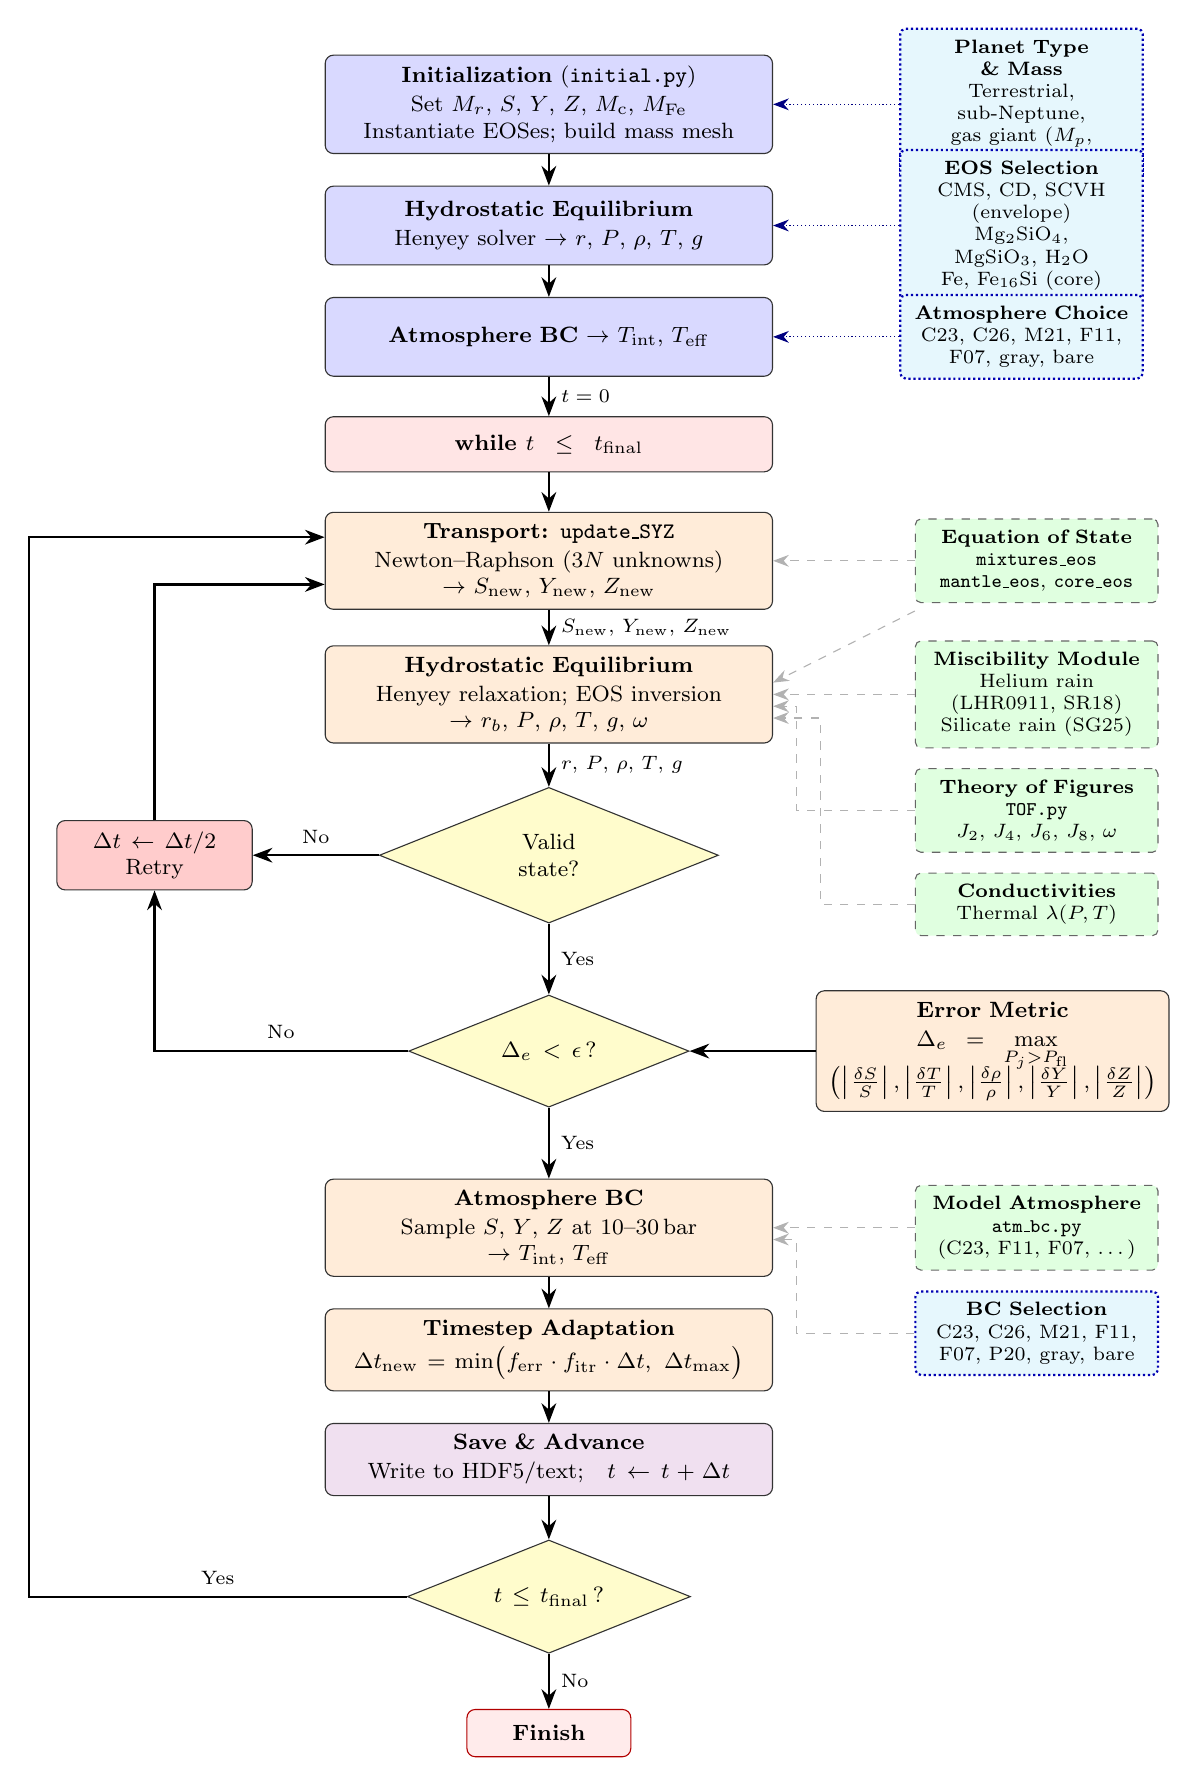
\begin{tikzpicture}[
    % ── Node styles ──
    init/.style={rectangle, draw=black!80, fill=blue!15, text width=5.4cm,
                 minimum height=1.0cm, align=center, rounded corners=3pt,
                 font=\footnotesize},
    process/.style={rectangle, draw=black!80, fill=orange!15, text width=5.4cm,
                    minimum height=0.9cm, align=center, rounded corners=3pt,
                    font=\footnotesize},
    decision/.style={diamond, draw=black!80, fill=yellow!20, text width=2.0cm,
                     minimum height=0.6cm, align=center, aspect=2.5,
                     font=\footnotesize},
    auxiliary/.style={rectangle, draw=black!60, fill=green!12, text width=2.8cm,
                      minimum height=0.6cm, align=center, rounded corners=2pt,
                      font=\scriptsize, dashed},
    userbox/.style={rectangle, draw=blue!70!black, fill=cyan!10, text width=2.8cm,
                    minimum height=0.6cm, align=center, rounded corners=2pt,
                    font=\scriptsize, densely dotted, thick},
    loopbox/.style={rectangle, draw=black!80, fill=red!10, text width=5.4cm,
                    minimum height=0.7cm, align=center, rounded corners=3pt,
                    font=\footnotesize\bfseries},
    retrybox/.style={rectangle, draw=black!80, fill=red!20, text width=2.2cm,
                     minimum height=0.7cm, align=center, rounded corners=3pt,
                     font=\footnotesize},
    savebox/.style={rectangle, draw=black!80, fill=violet!12, text width=5.4cm,
                    minimum height=0.8cm, align=center, rounded corners=3pt,
                    font=\footnotesize},
    finishbox/.style={rectangle, draw=red!70!black, fill=red!8, text width=1.8cm,
                      minimum height=0.6cm, align=center, rounded corners=3pt,
                      font=\footnotesize\bfseries},
    % ── Arrow styles ──
    arrow/.style={-{Stealth[length=2.5mm]}, thick},
    dasharrow/.style={-{Stealth[length=2mm]}, dashed, gray!60},
    dotarrow/.style={-{Stealth[length=2mm]}, densely dotted, blue!50!black},
    every node/.append style={inner sep=4pt},
]

% ============================
% COLUMN 1: INITIALIZATION
% ============================

\node[init] (init) {
    \textbf{Initialization} (\texttt{initial.py})\\[1pt]
    Set $M_r$, $S$, $Y$, $Z$, $M_{\rm c}$, $M_{\rm Fe}$\\
    Instantiate EOSes; build mass mesh
};

\node[init, below=0.4cm of init] (inithse) {
    \textbf{Hydrostatic Equilibrium}\\[1pt]
    Henyey solver $\rightarrow$ $r$, $P$, $\rho$, $T$, $g$
};

\node[init, below=0.4cm of inithse] (initbc) {
    \textbf{Atmosphere BC} $\rightarrow$ $T_{\rm int}$, $T_{\rm eff}$
};

% ============================
% USER CONFIG BOXES (right of init, cyan/dotted)
% ============================

\node[userbox, right=1.6cm of init] (planettype) {
    \textbf{Planet Type \& Mass}\\
    Terrestrial, sub-Neptune,\\
    gas giant ($M_p$, $M_{\rm c}$, $M_{\rm Fe}$)
};

\node[userbox, right=1.6cm of inithse] (eoschoice) {
    \textbf{EOS Selection}\\
    CMS, CD, SCVH (envelope)\\
    Mg$_2$SiO$_4$, MgSiO$_3$, H$_2$O\\
    Fe, Fe$_{16}$Si (core)
};

\node[userbox, right=1.6cm of initbc] (bcchoice) {
    \textbf{Atmosphere Choice}\\
    C23, C26, M21, F11,\\
    F07, gray, bare
};

% ============================
% MAIN LOOP
% ============================

\node[loopbox, below=0.5cm of initbc] (loopstart) {
    \textbf{while} $t \leq t_{\rm final}$
};

% Step 1: Transport
\node[process, below=0.5cm of loopstart] (transport) {
    \textbf{Transport:} \texttt{update\_SYZ}\\[1pt]
    Newton--Raphson ($3N$ unknowns)\\
    $\rightarrow$ $S_{\rm new}$, $Y_{\rm new}$, $Z_{\rm new}$
};

% Step 2: HSE
\node[process, below=0.45cm of transport] (hydro) {
    \textbf{Hydrostatic Equilibrium}\\[1pt]
    Henyey relaxation; EOS inversion\\
    $\rightarrow$ $r_b$, $P$, $\rho$, $T$, $g$, $\omega$
};

% Step 3: Validate
\node[decision, below=0.55cm of hydro] (validate) {
    Valid\\state?
};

% Step 4+5: Error
\node[decision, below=0.9cm of validate] (errcheck) {
    $\Delta_e < \epsilon$\,?
};

% Retry box (close enough that loop-back line passes to its left)
\node[retrybox, left=1.6cm of validate] (retry) {
    $\Delta t \leftarrow \Delta t / 2$\\
    Retry
};

% Error computation (right of errcheck)
\node[process, right=1.6cm of errcheck, text width=4.2cm] (errcomp) {
    \textbf{Error Metric}\\[1pt]
    $\Delta_e = \max\limits_{P_j > P_{\rm fl}}$\\[-3pt]
    $\left(\left|\frac{\delta S}{S}\right|,
    \left|\frac{\delta T}{T}\right|,
    \left|\frac{\delta \rho}{\rho}\right|,
    \left|\frac{\delta Y}{Y}\right|,
    \left|\frac{\delta Z}{Z}\right|\right)$
};

% Step 6: Atm BC
\node[process, below=0.9cm of errcheck] (atmbc) {
    \textbf{Atmosphere BC}\\[1pt]
    Sample $S$, $Y$, $Z$ at 10--30\,bar\\
    $\rightarrow$ $T_{\rm int}$, $T_{\rm eff}$
};

% Timestep adapt
\node[process, below=0.4cm of atmbc] (dtadapt) {
    \textbf{Timestep Adaptation}\\[1pt]
    $\Delta t_{\rm new} = \min\!\big(f_{\rm err}\cdot f_{\rm itr}\cdot \Delta t,\;\Delta t_{\rm max}\big)$
};

% Save & advance
\node[savebox, below=0.4cm of dtadapt] (save) {
    \textbf{Save \& Advance}\\[1pt]
    Write to HDF5/text;\quad $t \leftarrow t + \Delta t$
};

% Time check
\node[decision, below=0.55cm of save] (timecheck) {
    $t \leq t_{\rm final}$\,?
};

% Finish
\node[finishbox, below=0.7cm of timecheck] (finish) {
    \textbf{Finish}
};

% ============================
% AUXILIARY MODULES (right)
% ============================

\node[auxiliary, right=1.8cm of transport] (eos) {
    \textbf{Equation of State}\\
    \texttt{mixtures\_eos}\\
    \texttt{mantle\_eos}, \texttt{core\_eos}
};

\node[auxiliary, right=1.8cm of hydro] (misc) {
    \textbf{Miscibility Module}\\
    Helium rain (LHR0911, SR18)\\
    Silicate rain (SG25)
};

\node[auxiliary, below=0.25cm of misc] (tof) {
    \textbf{Theory of Figures}\\
    \texttt{TOF.py}\\
    $J_2$, $J_4$, $J_6$, $J_8$, $\omega$
};

\node[auxiliary, below=0.25cm of tof] (cond) {
    \textbf{Conductivities}\\
    Thermal $\lambda(P,T)$
};

\node[auxiliary, right=1.8cm of atmbc] (atm) {
    \textbf{Model Atmosphere}\\
    \texttt{atm\_bc.py}\\
    (C23, F11, F07, \ldots)
};

\node[userbox, below=0.25cm of atm] (atmselect) {
    \textbf{BC Selection}\\
    C23, C26, M21, F11,\\
    F07, P20, gray, bare
};

% ============================
% ARROWS: MAIN FLOW
% ============================

\draw[arrow] (init) -- (inithse);
\draw[arrow] (inithse) -- (initbc);
\draw[arrow] (initbc) -- node[right, font=\scriptsize] {$t=0$} (loopstart);
\draw[arrow] (loopstart) -- (transport);
\draw[arrow] (transport) -- node[right, font=\scriptsize] {$S_{\rm new}$, $Y_{\rm new}$, $Z_{\rm new}$} (hydro);
\draw[arrow] (hydro) -- node[right, font=\scriptsize] {$r$, $P$, $\rho$, $T$, $g$} (validate);
\draw[arrow] (validate) -- node[right, font=\scriptsize] {Yes} (errcheck);
\draw[arrow] (errcheck) -- node[right, font=\scriptsize] {Yes} (atmbc);
\draw[arrow] (atmbc) -- (dtadapt);
\draw[arrow] (dtadapt) -- (save);
\draw[arrow] (save) -- (timecheck);
\draw[arrow] (timecheck) -- node[right, font=\scriptsize] {No} (finish);

% ── Reject paths ──
% "No" from validate goes left to retry
\draw[arrow] (validate.west) -- node[above, font=\scriptsize] {No} (retry);
% "No" from errcheck goes left-up to retry
\draw[arrow] (errcheck.west) -| node[above left, font=\scriptsize, pos=0.2] {No} (retry);
% Retry arrow goes up and enters transport LOW on the left side
\draw[arrow] (retry.north) |- ([yshift=-0.3cm]transport.west);

% Loop-back from timecheck: route far left (beyond retry box), enter transport HIGH on left side
\draw[arrow] (timecheck.west) -- node[above, font=\scriptsize] {Yes}
    ++(-4.8,0) |- ([yshift=0.3cm]transport.west);

% ── Error computation ──
\draw[arrow] (errcomp.west) -- (errcheck.east);

% ============================
% ARROWS: AUXILIARY (dashed)
% ============================

\draw[dasharrow] (eos.west) -- (transport.east);
\draw[dasharrow] (misc.west) -- (hydro.east);
\draw[dasharrow] ([yshift=-0.1cm]eos.south west) -- ([yshift=0.15cm]hydro.east);
\draw[dasharrow] (tof.west) -| ([xshift=0.3cm, yshift=-0.15cm]hydro.east) -- ([yshift=-0.15cm]hydro.east);
\draw[dasharrow] (cond.west) -| ([xshift=0.6cm, yshift=-0.3cm]hydro.east) -- ([yshift=-0.3cm]hydro.east);
\draw[dasharrow] (atm.west) -- (atmbc.east);
\draw[dasharrow] (atmselect.west) -| ([xshift=0.3cm, yshift=-0.15cm]atmbc.east) -- ([yshift=-0.15cm]atmbc.east);

% ============================
% ARROWS: USER CONFIG (dotted, to init boxes)
% ============================

\draw[dotarrow] (planettype.west) -- (init.east);
\draw[dotarrow] (eoschoice.west) -- (inithse.east);
\draw[dotarrow] (bcchoice.west) -- (initbc.east);

\end{tikzpicture}

\end{document}
